\paragraph{GET /:lang/user/training/question} % richiesta che ritorna la prossima domanda dell'allenamento
\begin{itemize}
\item \textbf{Successo}: questo scenario rappresenta il successo di una richiesta che ritorna la domanda successiva nella modalità allenamento. In questo caso il modulo \texttt{TopicController} invia \texttt{next()} per indicare il successo dell'operazione.

\begin{figure}[ht]
	\centering
	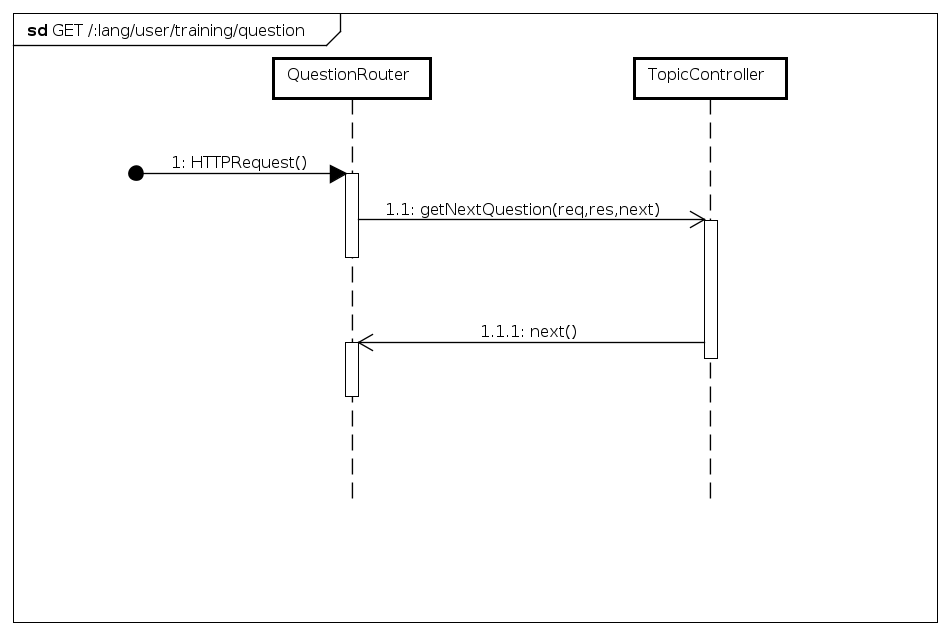
\includegraphics[scale=0.45]{UML/DiagrammiDiSequenza/Back-end/GET__lang_user_training_question_success.png}
	\caption{Procedura di restituzione della domanda successiva nella modalità allenamento}
\end{figure}
\FloatBarrier

\item \textbf{Fallimento}: questo scenario rappresenta il fallimento di una richiesta che ritorna la domanda successiva nella modalità allenamento; in questo caso il modulo \texttt{TopicController} ritornerà un \texttt{next(err)} al router che avrà il compito di reinstradarlo (indirizzandolo verso \texttt{ErrorHandler}).

\begin{figure}[ht]
	\centering
	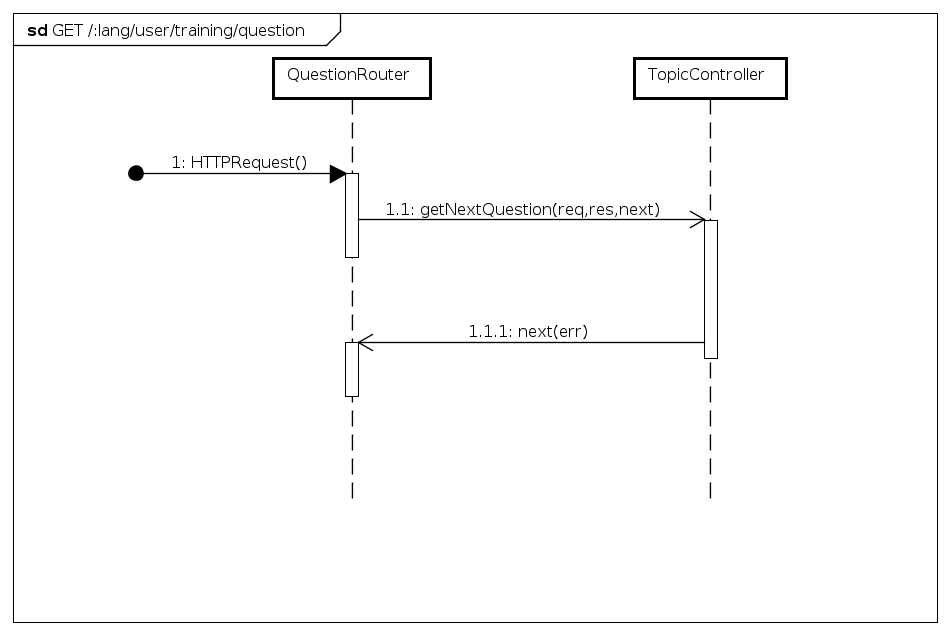
\includegraphics[scale=0.45]{UML/DiagrammiDiSequenza/Back-end/GET__lang_user_training_question_failure.png}
	\caption{Fallimento della procedura di restituzione della domanda successiva nella modalità allenamento}
\end{figure}
\FloatBarrier

\end{itemize}


\paragraph{PUT /:lang/user/:userId/training/userstatistics} % richiesta che aggiorna le statistiche dell'utente
\begin{itemize}
\item \textbf{Successo}: questo scenario rappresenta il successo di una richiesta aggiorna le statistiche di un utente dopo che ha risposto ad una domanda che impone, come vincolo per poter essere effettuata, che l'utente sia autenticato al sistema; quindi prima di tale operazione deve venire fatta una richiesta di controllo di sessione mediante l'apposita risorsa \textit{REST\ped{G}}. In questo caso il modulo \texttt{UserManagementController} invia \texttt{next()} per indicare il successo dell'operazione.

\begin{figure}[ht]
	\centering
	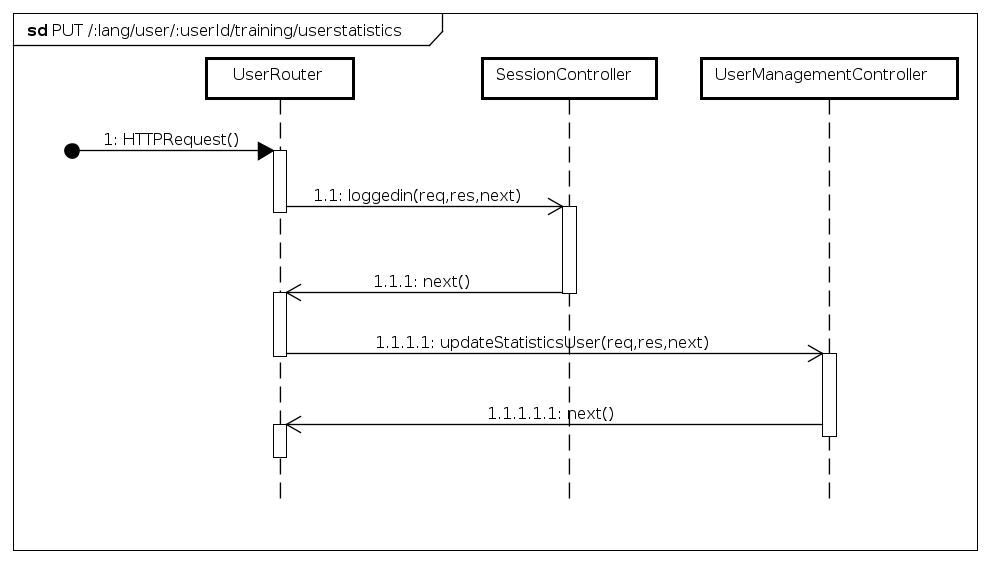
\includegraphics[scale=0.45]{UML/DiagrammiDiSequenza/Back-end/PUT__lang_user__userId_training_userstatistics_success.png}
	\caption{Procedura di aggiornamento delle statistiche dell'utente dopo una risposta ad una domanda}
\end{figure}
\FloatBarrier

\item \textbf{Fallimento}: questo scenario rappresenta il fallimento di una richiesta che aggiorna le statistiche di un utente dopo che ha risposto ad una domanda che impone, come vincolo per poter essere effettuata, che l'utente sia autenticato al sistema; quindi prima di tale operazione deve venire fatta una richiesta di controllo di sessione mediante l'apposita risorsa \textit{REST\ped{G}}. In questo caso il modulo \texttt{UserManagementController} invia \texttt{next(error)} per indicare il fallimento di tale vincolo al router il quale avrà compito di reinstradarlo (indirizzandolo verso \texttt{ErrorHandler}).

\begin{figure}[ht]
	\centering
	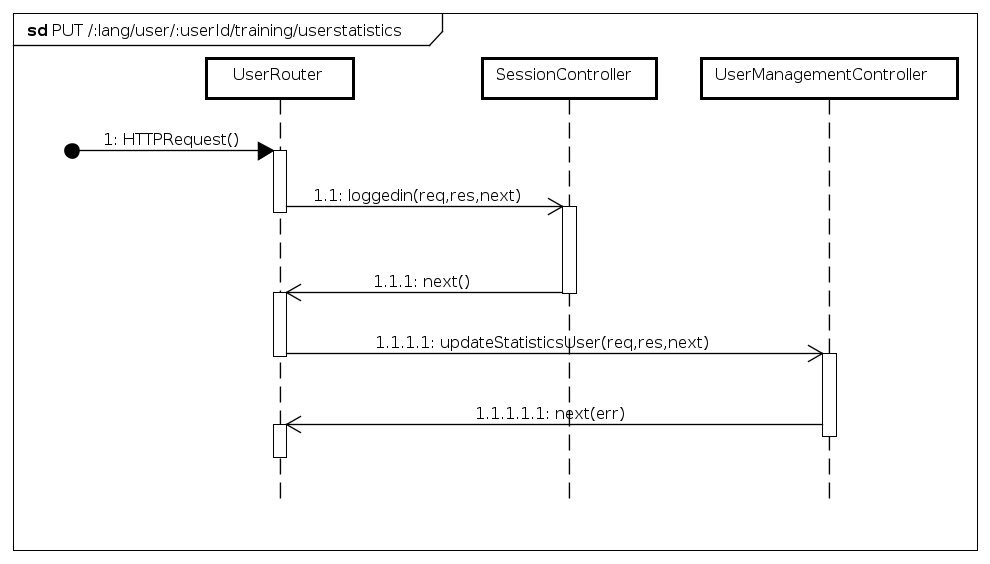
\includegraphics[scale=0.45]{UML/DiagrammiDiSequenza/Back-end/PUT__lang_user__userId_training_userstatistics_failure.png}
	\caption{Fallimento della procedura di aggiornamento delle statistiche dell'utente dopo una risposta ad una domanda}
\end{figure}
\FloatBarrier

\end{itemize}


\paragraph{PUT /:lang/user/:userId/training/questionstatistics} % richiesta che aggiorna le statistiche della domanda
\begin{itemize}
\item \textbf{Successo}: questo scenario rappresenta il successo di una richiesta aggiorna le statistiche di una domanda a cui è stata data una risposta che impone, come vincolo per poter essere effettuata, che l'utente sia autenticato al sistema; quindi prima di tale operazione deve venire fatta una richiesta di controllo di sessione mediante l'apposita risorsa \textit{REST\ped{G}}. In questo caso il modulo \texttt{QuestionController} invia \texttt{next()} per indicare il successo dell'operazione.

\begin{figure}[ht]
	\centering
	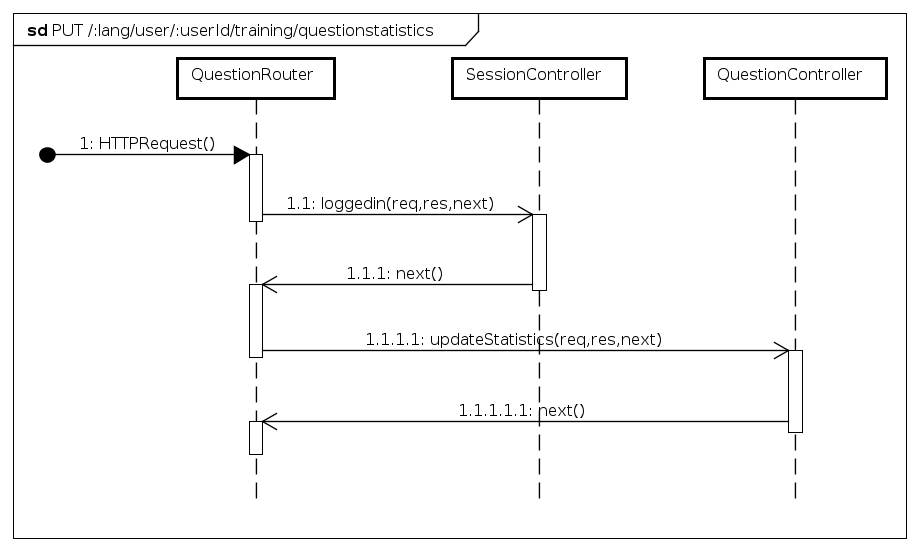
\includegraphics[scale=0.45]{UML/DiagrammiDiSequenza/Back-end/PUT__lang_user__userId_training_questionstatistics_success.png}
	\caption{Procedura di aggiornamento delle statistiche di una domanda}
\end{figure}
\FloatBarrier

\item \textbf{Fallimento}: questo scenario rappresenta il fallimento di una richiesta che aggiorna le statistiche di una domanda a cui è appena stata data una risposta che impone, come vincolo per poter essere effettuata, che l'utente sia autenticato al sistema; quindi prima di tale operazione deve venire fatta una richiesta di controllo di sessione mediante l'apposita risorsa \textit{REST\ped{G}}. In questo caso il modulo \texttt{QuestionController} invia \texttt{next(error)} per indicare il fallimento di tale vincolo al router il quale avrà compito di reinstradarlo (indirizzandolo verso \texttt{ErrorHandler}).

\begin{figure}[ht]
	\centering
	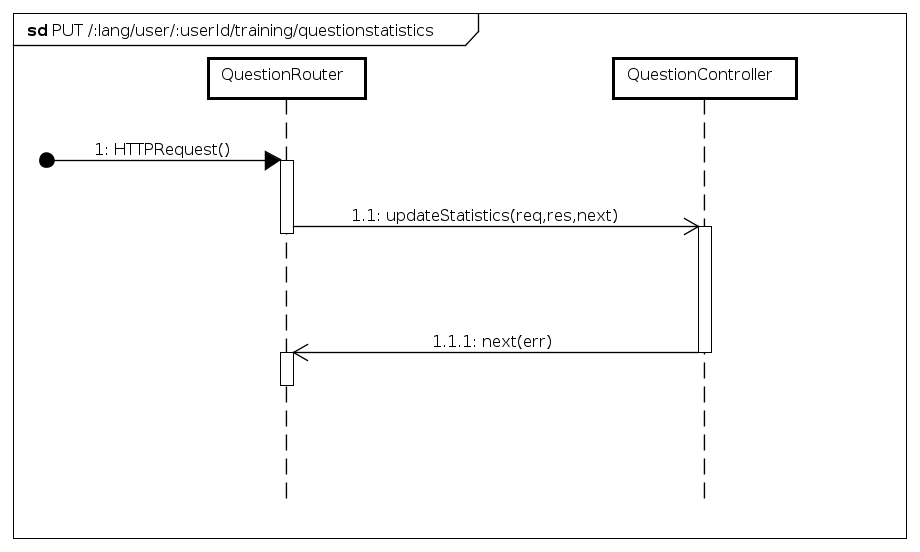
\includegraphics[scale=0.45]{UML/DiagrammiDiSequenza/Back-end/PUT__lang_user__userId_training_questionstatistics_failure.png}
	\caption{Fallimento della procedura di aggiornamento delle statistiche di una domanda}
\end{figure}
\FloatBarrier

\end{itemize} 

\paragraph{PUT /:lang/user/training/userlevelupdate}
\begin{itemize}
\item \textbf{Successo}: questo scenario rappresenta il successo di una richiesta che aggiorna il livello di un utente non autenticato per far sì che il sistema scelga domande adeguate alla sua preparazione. In questo caso il modulo \texttt{UserManagementController} invia \texttt{next()} per indicare il successo dell'operazione.

\begin{figure}[ht]
	\centering
	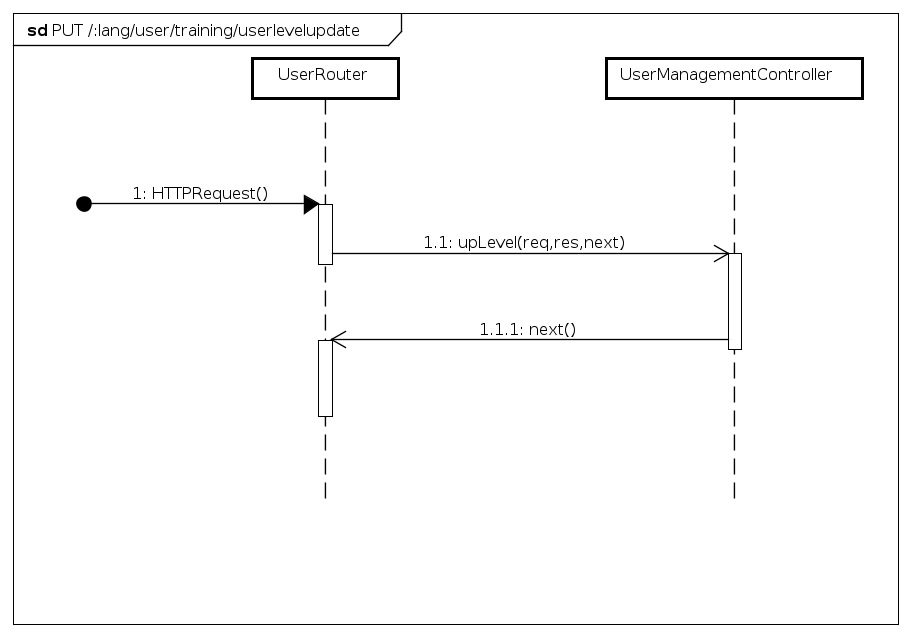
\includegraphics[scale=0.45]{UML/DiagrammiDiSequenza/Back-end/PUT__lang_user_training_userlevelupdate_success.png}
	\caption{Procedura di aggiornamento del livello di un utente non autenticato}
\end{figure}
\FloatBarrier

\item \textbf{Fallimento}: questo scenario rappresenta il fallimento una richiesta che aggiorna il livello di un utente non autenticato. In questo caso il modulo \texttt{UserManagementController} ritornerà un \texttt{next(err)} al router che avrà il compito di reinstradarlo (indirizzandolo verso \texttt{ErrorHandler}).

\begin{figure}[ht]
	\centering
	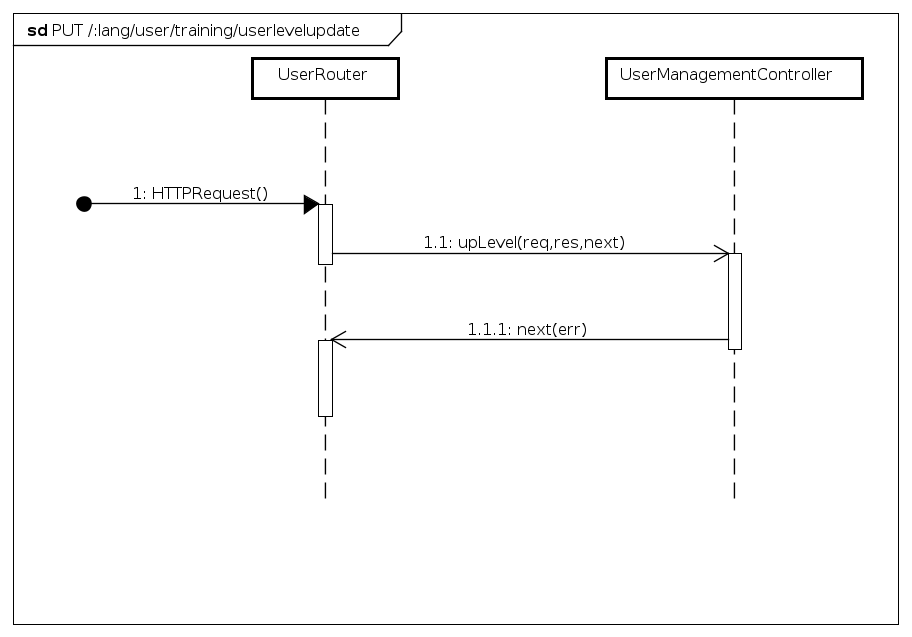
\includegraphics[scale=0.45]{UML/DiagrammiDiSequenza/Back-end/PUT__lang_user_training_userlevelupdate_failure.png}
	\caption{Fallimento della procedura di aggiornamento del livello di un utente non autenticato}
\end{figure}
\FloatBarrier

\end{itemize} 